
\section{Ameaças à Validade}

Alguns pontos do trabalho não têm o devido respaldo científico: o mesmo
parâmetro de Poisson para diferentes versões da aplicação instrumentada; a
distribuição uniforme de arestas; e o mesmo parâmetro de Poisson para descrever
o número médio de falhas por execução para todos os vértices.

As duas primeiras Leis de Lehman --- Lei da Mudança Contínua e Lei da
Complexidade Crescente --- evidenciam que o software sofre alterações e que sua
complexidade aumenta ao longo do seu ciclo de vida \cite{Wazlawick2013}. O
resultado prático é o crescimento contra-intuitivo da taxa de falhas global do
sistema, bem como a aparição de picos de falhas após manutenção do mesmo
(figura \ref{Figure061-FailureRate}).

\hfill \break
{
  \centering
  \captionsetup{type=figure}
	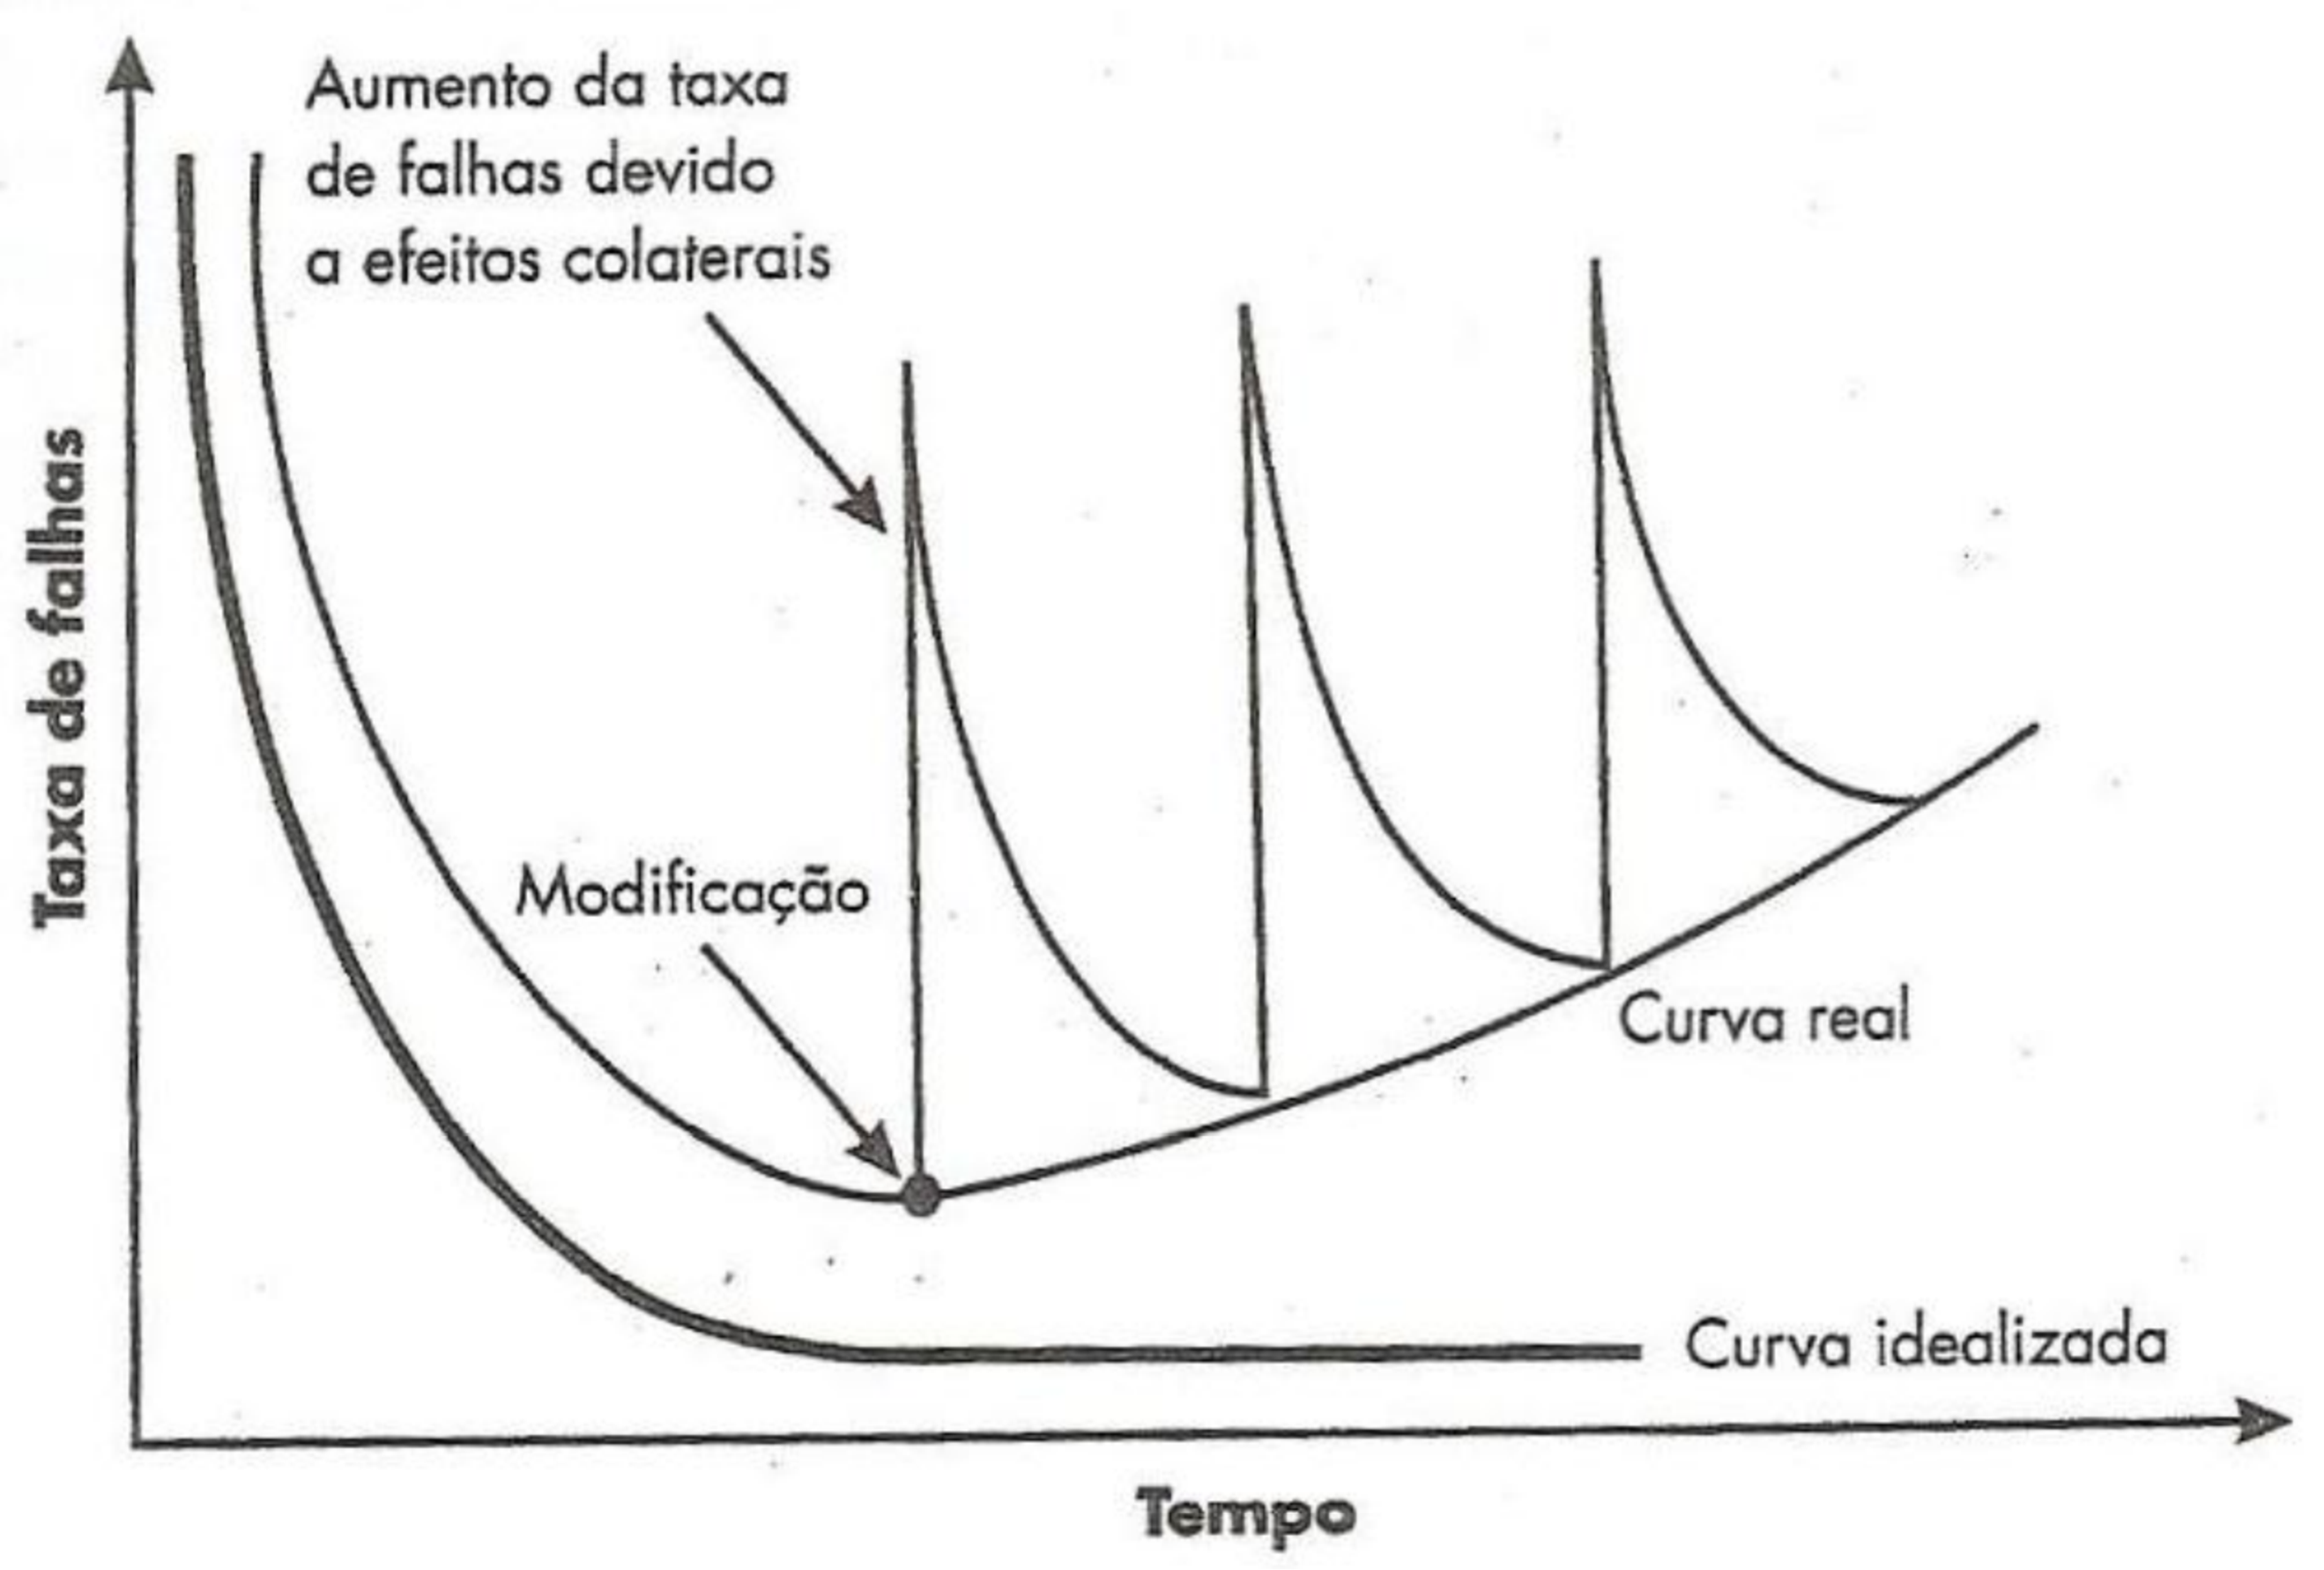
\includegraphics[scale=0.1625]{./figures/Figure061-FailureRate.pdf}
  \captionof{figure}{
    evolução da taxa de falha idealizada e real para sistemas de software.
    Atividades de manuteção muitas vezes resultam em um aumento da taxa de
    falhas, à medida que erros são inseridos e a arquitetura do sistema se
    deteriora.
  }
  \hfill
	\label{Figure061-FailureRate}
}

Os graus de acoplamento e coesão e a complexidade de um determinado trecho de
código provavelmente se relacionam com o grau do vértice correspondente no grafo
mapa. A distribuição uniforme de arestas com probabilidade $p=0,5$ não parece
plausível.

Ademais, um alto grau de acoplamento, baixo grau de coesão e alta complexidade
são fatores que favorecem alta taxa de falhas para componentes de software. Do
contrário, baixo grau de acoplamento, alto grau de coesão e baixa complexidade
são fatores que favorecem baixa taxa de falhas para um componente de software.
Em análise preliminar, parece abusivo assumir que todos os componentes
apresentarão a mesma susceptibilidade a falhas (parâmetro de Poisson).
